\documentclass[12pt,a4paper]{article}
\usepackage[a4paper, margin=2cm]{geometry}
\usepackage{amsmath}
\usepackage{fancyhdr}
\usepackage{graphicx}
\usepackage{pdflscape}
\usepackage{svg}
\usepackage{hyperref}
\usepackage{enumitem}
\usepackage[absolute,overlay]{textpos}
\usepackage{lipsum}
\usepackage{amssymb}

\newcommand{\reporttitle}{Homework 1}
\newcommand{\authorname}{Afonso da Conceição Ribeiro}
\newcommand{\authorid}{ist1102763}
\newcommand{\authorgroup}{Grupo 86}
\newcommand{\istul}{Instituto Superior Técnico -- Universidade de Lisboa}
\newcommand{\reportcourse}{Aprendizagem Profunda}
\newcommand{\reportyear}{2024/2025}

\newcommand{\m}[1]{\mathbf{#1}}

\hypersetup{
    colorlinks=true,
    linkcolor=blue,
    filecolor=magenta,
    urlcolor=blue,
    citecolor=blue,
    pdftitle={\reporttitle},
    pdfpagemode=FullScreen,
}

\pagestyle{fancy}
\fancyhf{}
\lhead{\reporttitle}
\rhead{\reportcourse}
\lfoot{\authorgroup}
\rfoot{\thepage}


\renewcommand{\footrulewidth}{0.2pt}

\renewcommand\thesection{\arabic{section}.}
\renewcommand\thesubsection{\thesection\arabic{subsection}.}
\renewcommand\thesubsubsection{\thesubsection\arabic{subsubsection}.}

\usepackage{etoolbox} % Necessário para modificar comandos
\makeatletter % Indentar parágrafos dentro de subseções
\preto\subsection{\setlength{\parindent}{2em}} % Ajusta o tamanho do recuo
\makeatother

\begin{document}
    \begin{titlepage}

        \begin{textblock*}{0cm}(10cm, 0cm)
            
\includegraphics[width=10cm]{Logo IST.jpg}
        \end{textblock*}

        \centering
        \vspace*{5cm}
        {\Huge \textbf{\reporttitle} \par}

        \vspace{0.5cm}
        {\LARGE \reportcourse \par}

        \vspace{0.5cm}
        {\large \reportyear \par}

        \vspace{2cm}
        {\large \authorgroup \par}
        
        \vspace{0.25cm}
        {\large \istul \par}

        \vfill
        \renewcommand{\contentsname}{Índice}
        \tableofcontents

        \thispagestyle{empty}
        \clearpage

    \end{titlepage}

    \section*{Contribution of each member of the group}
    All members of the group participated in every stage of this homework. Each member contributed equally to implementing the code, analyzing the results and writing the report.

    \setcounter{page}{2}
    \setcounter{secnumdepth}{0} % Disable numbering for sections and below
    \setlength{\parskip}{0em}

    \newlength{\imagewidth} % Declare a new length
    \setlength{\imagewidth}{8cm} % Set its value


    \section{Question 1}
    \subsection{1. a)}
        Plot of the train and validation accuracies as a function of the epoch number: \\
        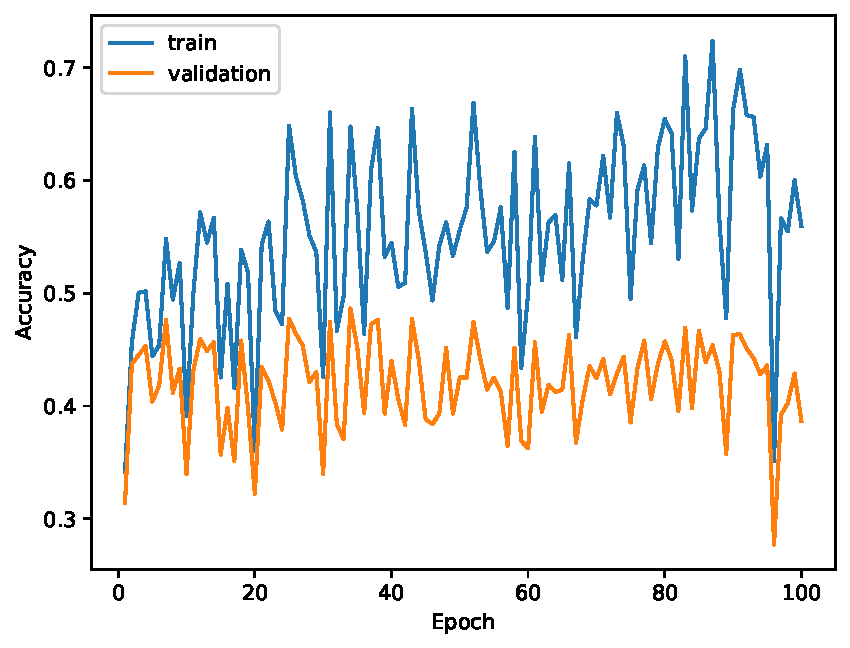
\includegraphics[width=\imagewidth]{q1/q1_1a-accs.pdf} \\
        Final test accuracy: 0.37433333333333335

    \subsection{2. a)}
        Plot of the train and validation accuracies as a function of the epoch number: \\
        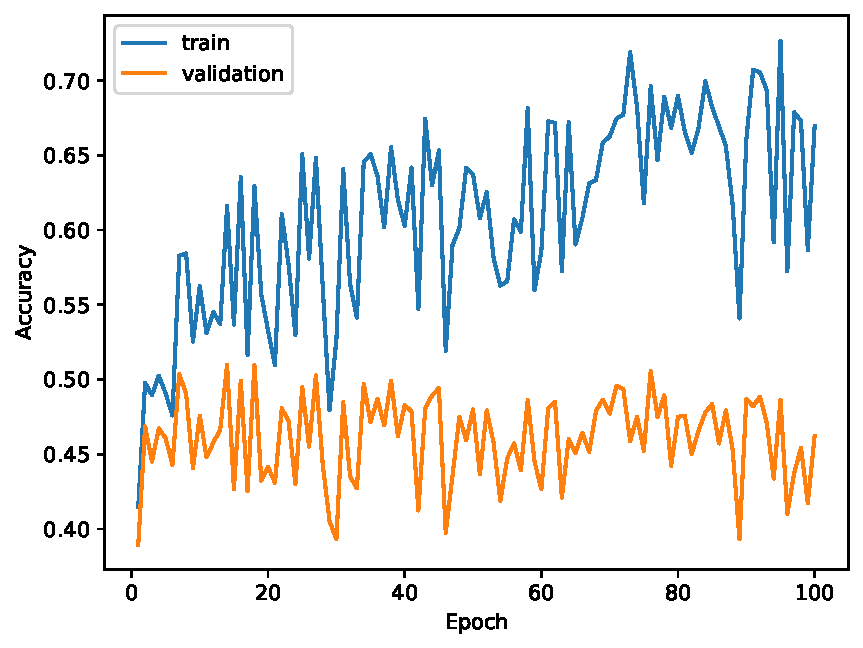
\includegraphics[width=\imagewidth]{q1/q1_2a-accs.pdf} \\
        Final test accuracy: 0.45966666666666667
    
    \subsection{2. b)}
        Plot of the train and validation accuracies as a function of the epoch number: \\
        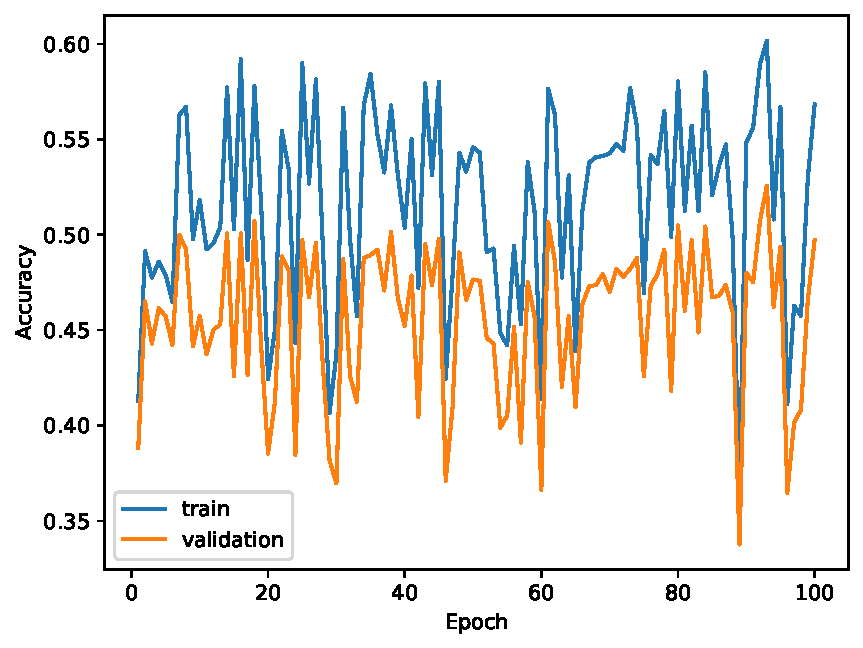
\includegraphics[width=\imagewidth]{q1/q1_2b-accs.pdf} \\
        Final test accuracy: 0.5053333333333333 \\
        We can see that the first classifier, trained with no regularization, has better train accuracy than the second one, trained with \(\ell_2\) regularization. This makes sense because, without \(\ell_2\) regularization, the first classifier is free to overfit the training data, which is evidenced by a notable gap between the train and validation accuracies in that model, compared to the smaller gap between the values of the second one. The validation and test accuracies are, as expected, larger in the \(\ell_2\)-regularized classifier, once the overfitting of the first one makes it harder for it to generalize to new data. The model with \(\ell_2\) regularization penalizes large weights, leading to smoother decision boundaries, which helps reduce overfitting and, as a consequence, generalize better to unseen data, and hence its larger test accuracy.

    \subsection{2. c)}
        Plot of the \(\ell_2\)-norm of the weights of the non-regularized (left) and the \(\ell_2\)-regularized (right) versions of the logistic regression classifiers as a function of the epoch number: \\
        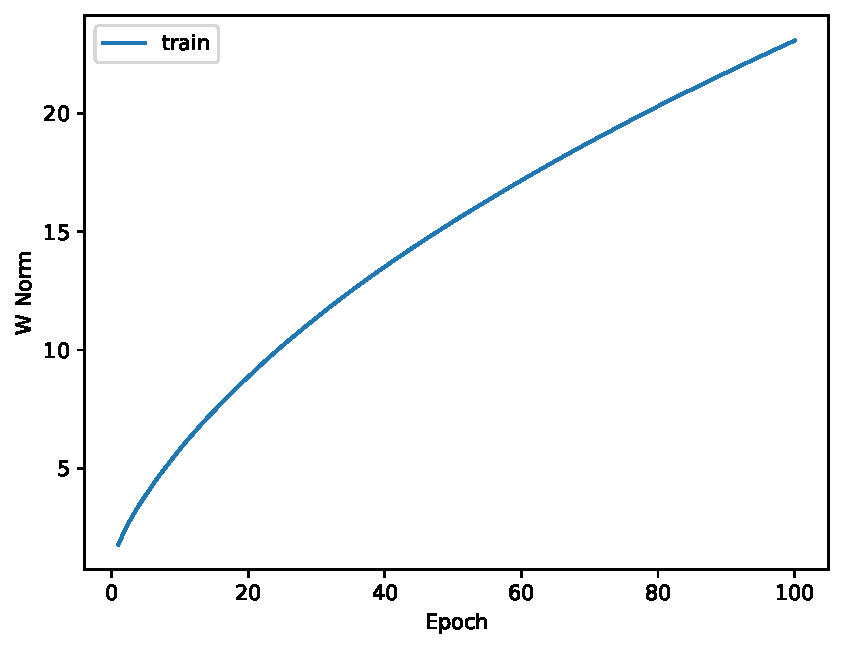
\includegraphics[width=\imagewidth]{q1/q1_2a-w_norms.pdf}
        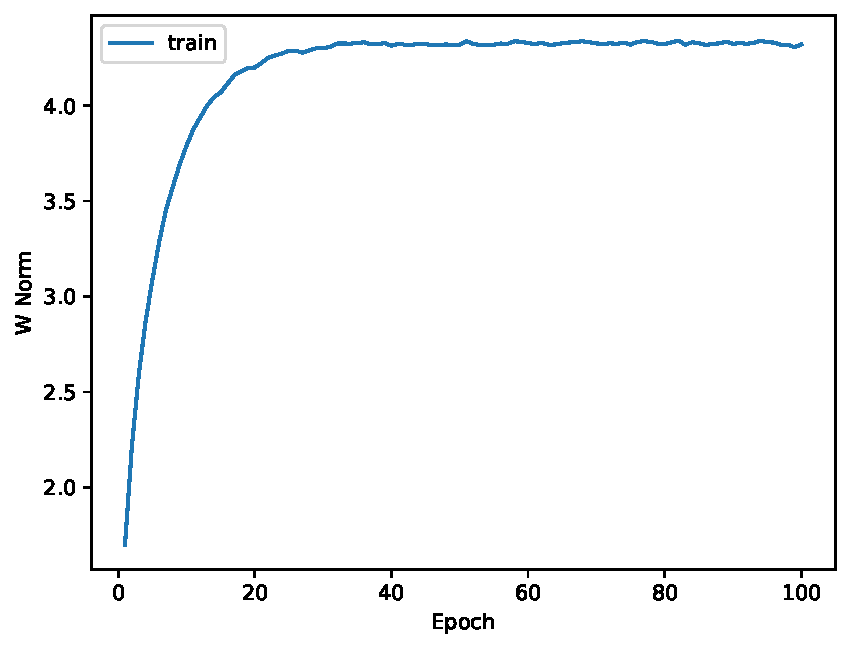
\includegraphics[width=\imagewidth]{q1/q1_2b-w_norms.pdf} \\
        The \(\ell_2\)-norm of the weights of the non-regularized classifier increases steadily and significantly over the epochs, which indicates that the model's parameters grow larger as it continues to minimize the loss without any constraints, leading to overfitting. On the other hand, for the \(\ell_2\)-regularized classifier, the \(\ell_2\)-norm stabilizes around the 20th epoch, at a much lower range (around 4.3) compared to the non-regularized case (which goes up to almost 25). This reflects the effect of \(\ell_2\)-regularization, which penalizes large weight values, thereby controlling the magnitude of the weights throughout training.

    \subsection{2. d)}      
        The \(\ell_1\) regularization adds a penalty proportional to the sum of the absolute values of the weights (\(\sum_{i,j} |W_{i,j}|\)), resulting in sparse weights, with some becoming zero. As a result, the model will rely on fewer features, effectively performing feature selection and focusing on the most important ones, but also sacrificing some of the nuanced information provided by less important features. In contrast, the \(\ell_2\) regularization adds a penalty proportional to the sum of the squares of the weights (\(\sum_{i,j} W_{i,j}^2\)), which discourages large weight magnitudes but does not drive weights to exactly zero. Instead, it spreads the impact across all features more evenly, reducing the risk of overfitting without completely eliminating features.

    \subsection{3. a)}
        Plot of the train and validation accuracies as a function of the epoch number: \\
        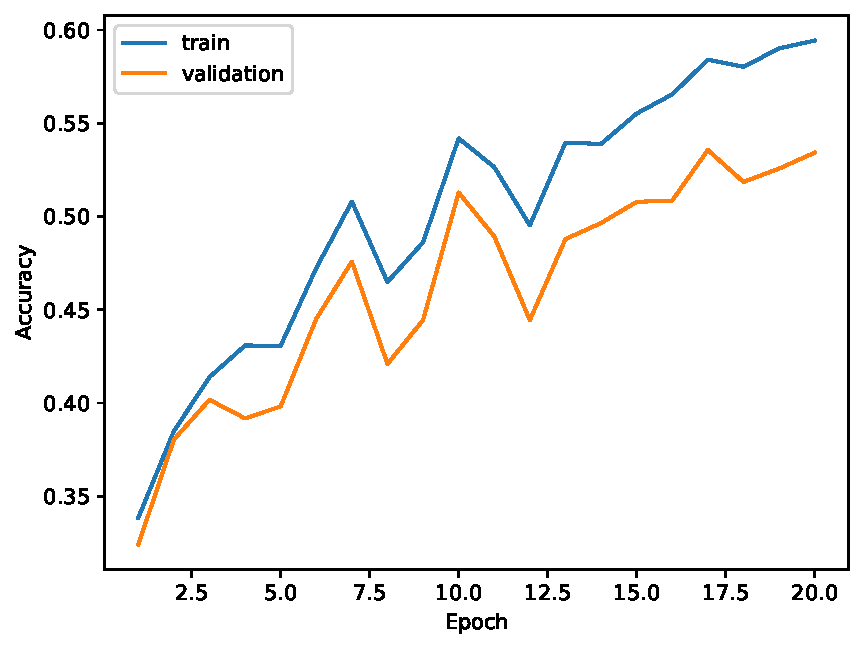
\includegraphics[width=\imagewidth]{q1/q1_3a-accs.pdf} \\
        Final test accuracy: 0.5443333333333333


    \newpage
    \section{Question 2}
    \subsection{1.}
        Plots of the train and validation losses (left) and the validation accuracy (right) as a function of the epoch number for the model trained with:
        \begin{itemize}
            \item Learning rate 0.00001: \\
                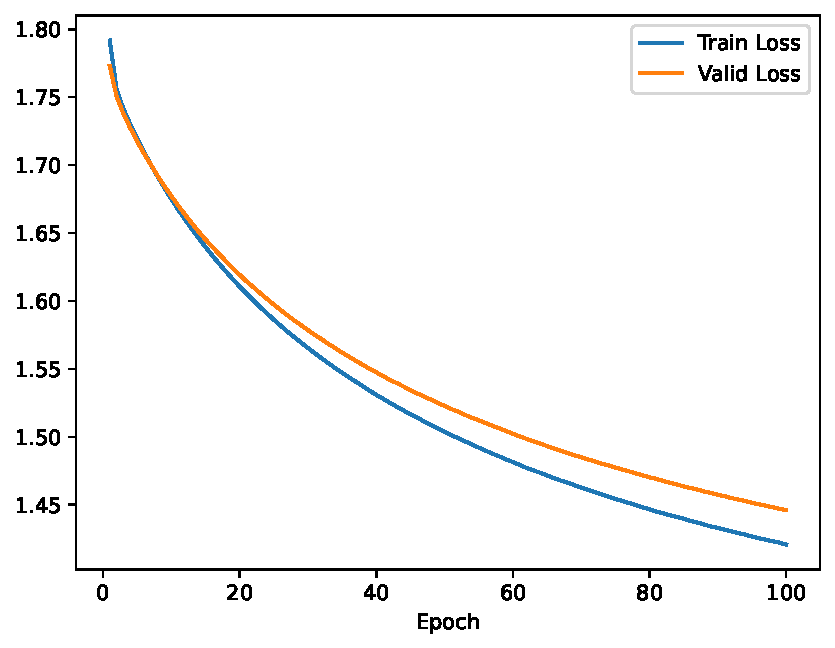
\includegraphics[width=\imagewidth]{q2/q2_1_lr-0.00001-training-loss.pdf}
                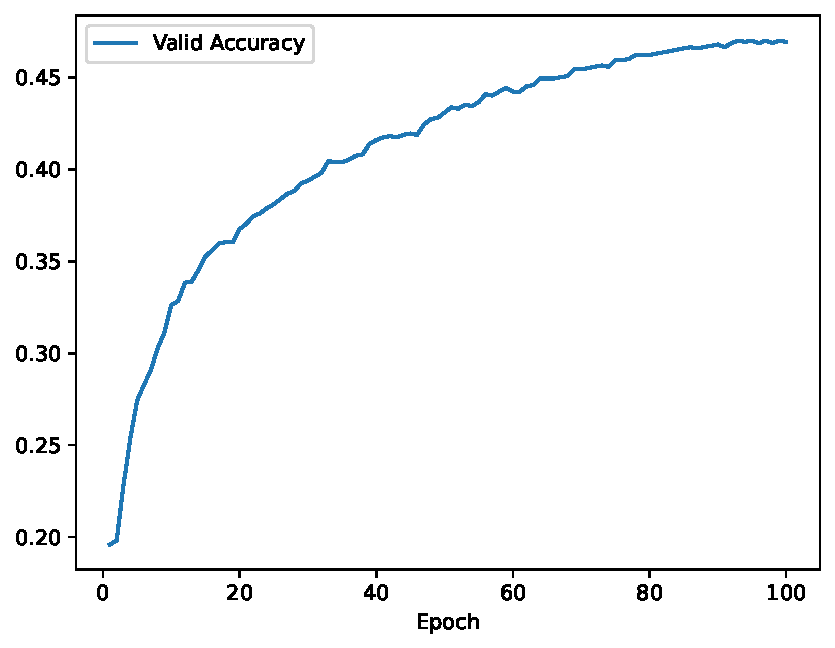
\includegraphics[width=\imagewidth]{q2/q2_1_lr-0.00001-validation-accuracy.pdf}
            \item Learning rate 0.001: \\
                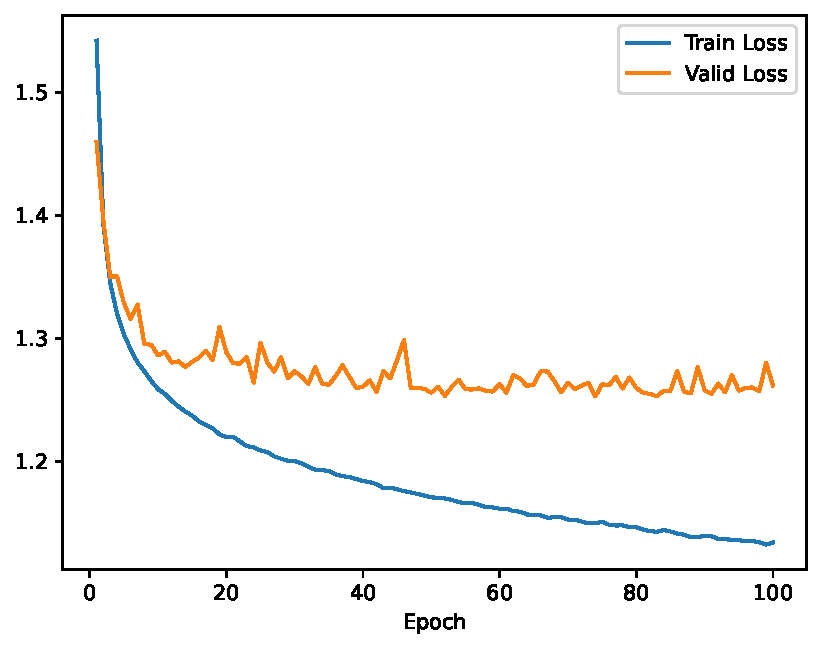
\includegraphics[width=\imagewidth]{q2/q2_1_lr-0.001-training-loss.pdf}
                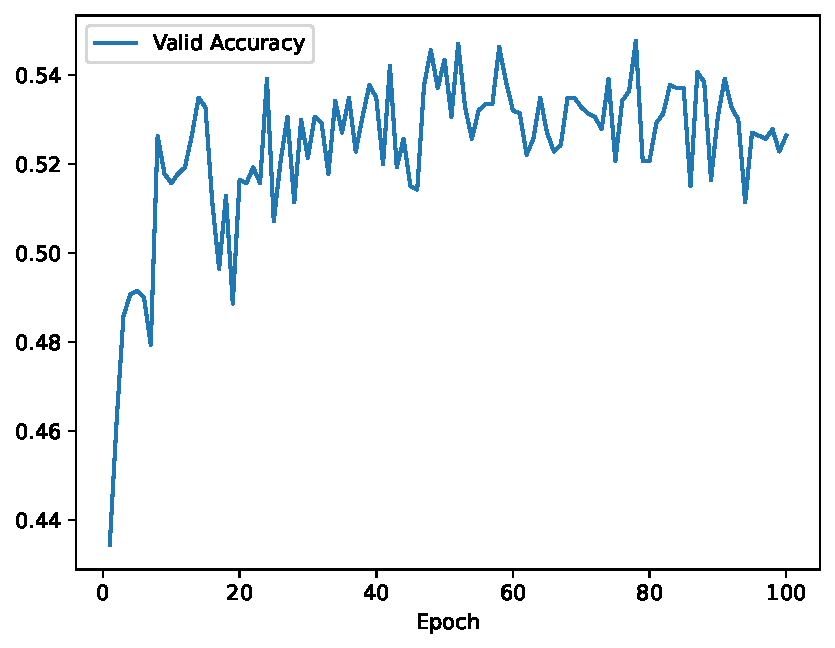
\includegraphics[width=\imagewidth]{q2/q2_1_lr-0.001-validation-accuracy.pdf}
            \item Learning rate 0.1: \\
                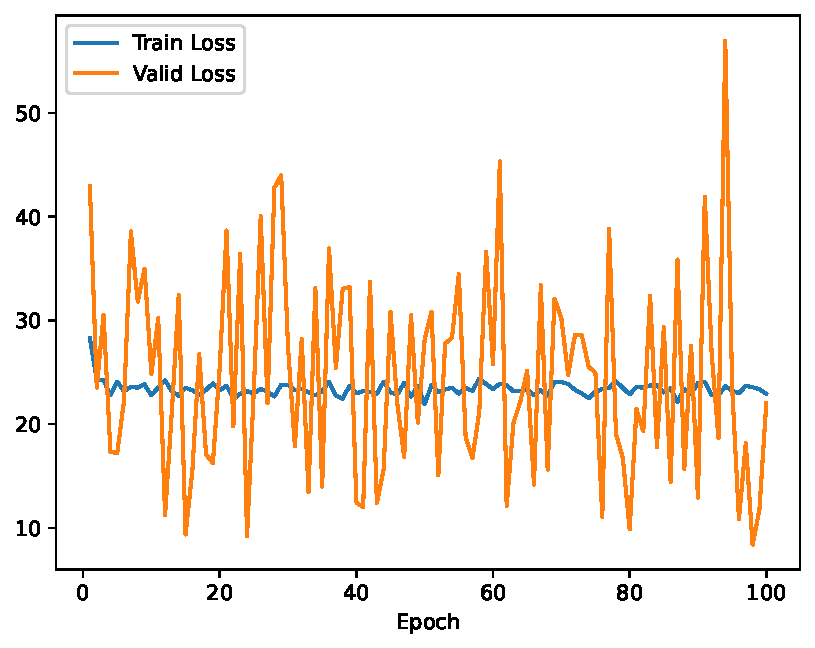
\includegraphics[width=\imagewidth]{q2/q2_1_lr-0.1-training-loss.pdf}
                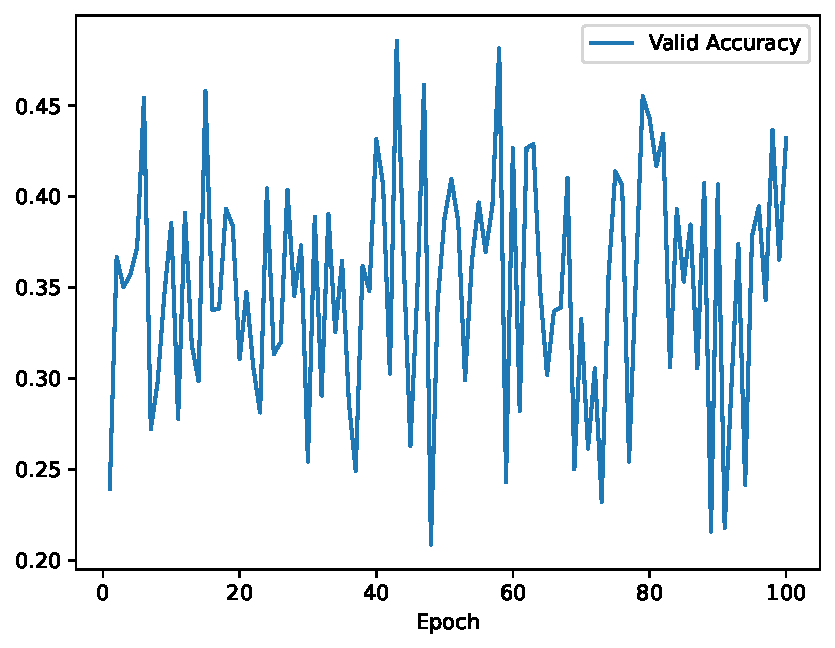
\includegraphics[width=\imagewidth]{q2/q2_1_lr-0.1-validation-accuracy.pdf}
        \end{itemize}
        \newpage
        \noindent With a learning rate of 0.00001, the training and validation losses decrease smoothly but very slowly, indicating that the model is converging at a very slow pace. While the loss reduces consistently, the validation accuracy plateaus around 0.45, showing that the learning rate is too small for the model to adjust effectively within the given number of epochs. \\
        As for the learning rate 0.001, the model achieves a good balance between speed and stability. The training loss decreases smoothly, and the validation loss stabilizes after an initial drop. The validation accuracy improves quickly, reaching around 0.52, which demonstrates efficient convergence without significant overfitting. \\
        Finally, for the learning rate 0.1, both the training and validation losses fluctuate wildly, and the validation accuracy remains unstable, varying between 0.2 and 0.5. This instability occurs because the large learning rate causes the optimizer to overshoot the loss minimum repeatedly, preventing the model from converging. \\
        With that being said, the learning rate 0.001 leads to the best performance, as it allows the model to converge efficiently and stably, while smaller and larger learning rates result in either very slow progress or unstable training, respectively.

    \newpage
    \subsection{2. a)}
        Plots of the train and validation losses (left) and the validation accuracy (right) as a function of the epoch number for the model trained with:
        \begin{itemize}
            \item Batch size 64: \\
                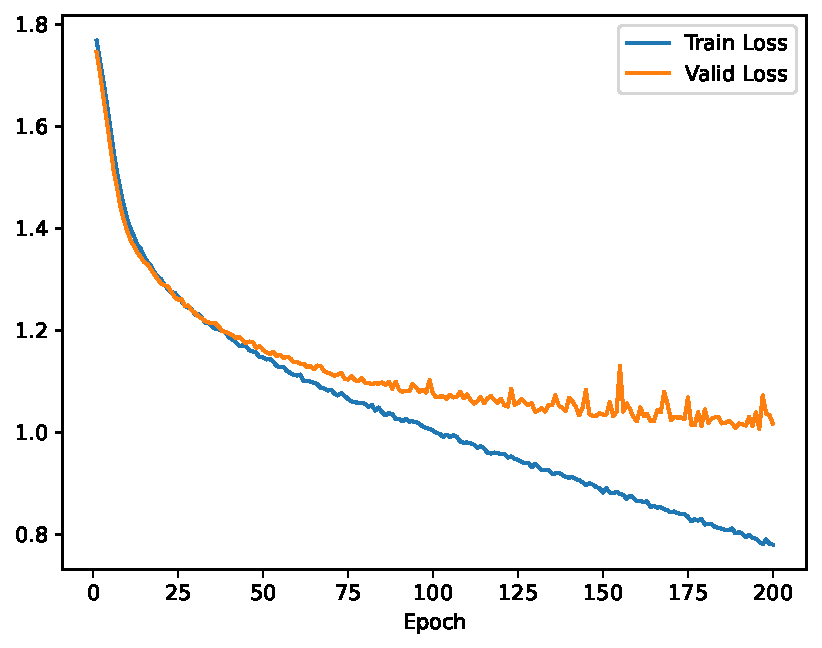
\includegraphics[width=\imagewidth]{q2/q2_2a_default-training-loss.pdf}
                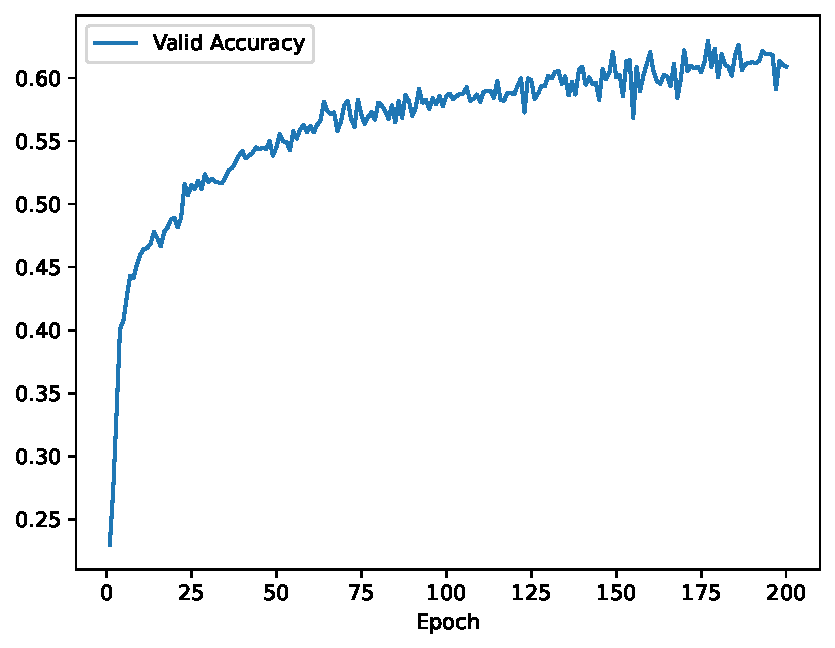
\includegraphics[width=\imagewidth]{q2/q2_2a_default-validation-accuracy.pdf} \\
                Test accuracy: 0.6080 \\
                Validation accuracy: 0.6090 \\
                Time of execution: 2 minutes and 45 seconds
            \item Batch size 512: \\
                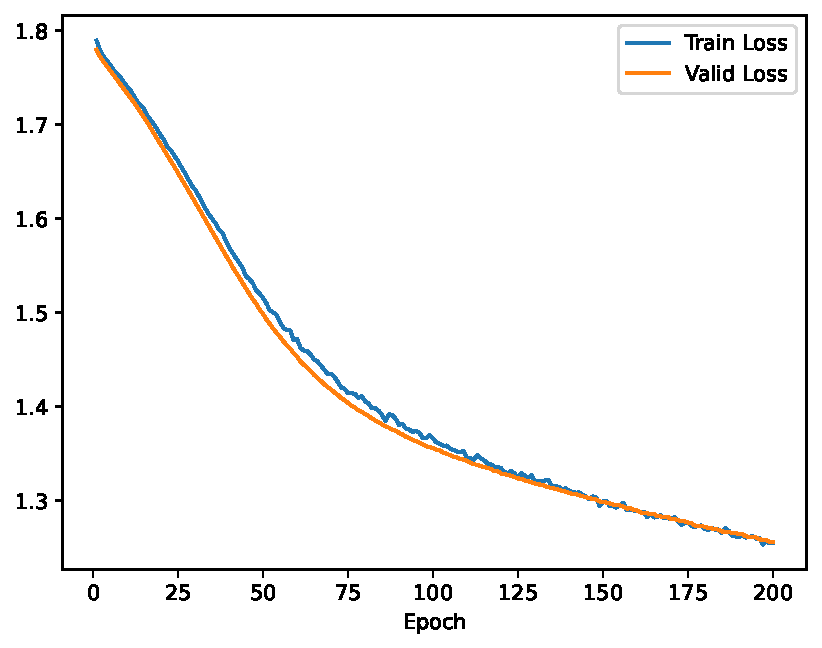
\includegraphics[width=\imagewidth]{q2/q2_2a_batch_512-training-loss.pdf}
                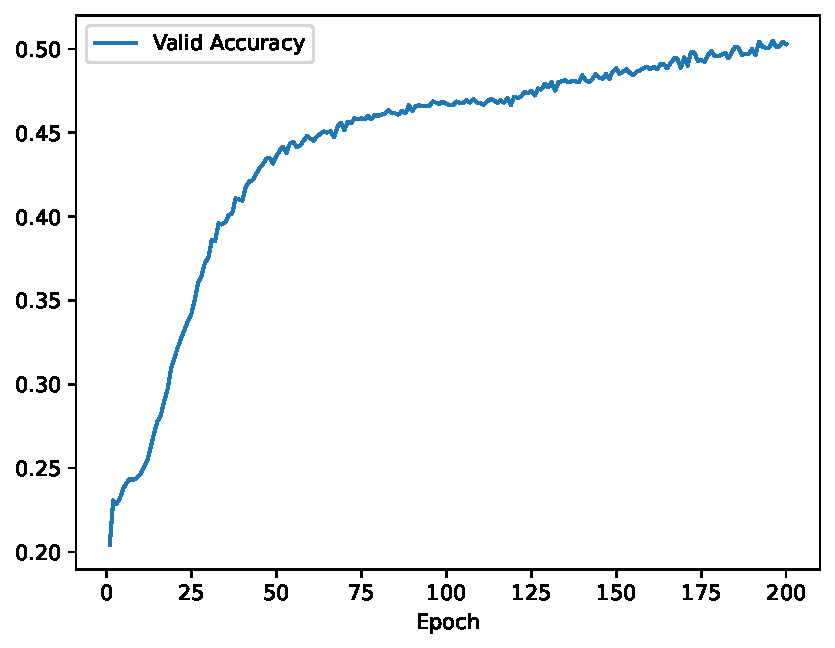
\includegraphics[width=\imagewidth]{q2/q2_2a_batch_512-validation-accuracy.pdf} \\
                Test accuracy: 0.5190 \\
                Validation accuracy: 0.5028 \\
                Time of execution: 1 minutes and 26 seconds
        \end{itemize}
        In the first model, the smaller batch size allowed for more frequent weight updates, leading to better convergence and improved generalization, as reflected in the higher accuracy. In contrast, the model with larger batch size reduced the frequency of updates, resulting in slower convergence and poorer generalization. The loss curves for batch size 64 show a steady decrease with a small gap between training and validation losses, indicating good learning and generalization. With batch size 512, the losses decrease uniformly but more slowly, suggesting underfitting due to smoother but less varied gradient updates. Training time also differed significantly: the larger batch size reduced computational time by requiring fewer updates per epoch, but at the cost of performance. In conclusion, the smaller batch size yields better accuracy and generalization, while the larger batch size trades off accuracy for faster execution.
    
    \subsection{2. b)}
        Plots of the train and validation losses (left) and the validation accuracy (right) as a function of the epoch number for the model trained with:
        \begin{itemize}
            \item Dropout 0.01: \\
                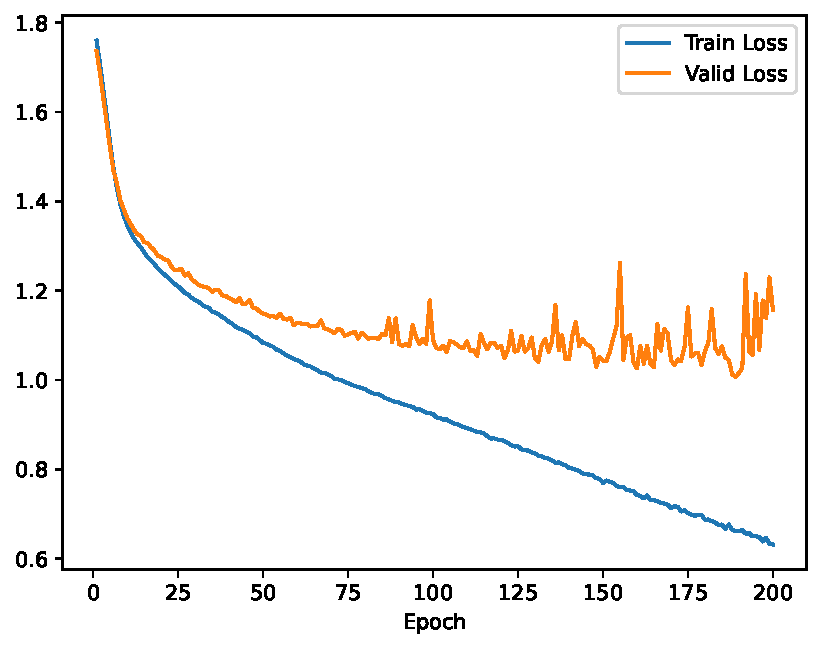
\includegraphics[width=\imagewidth]{q2/q2_2b_dropout_0.01-training-loss.pdf}
                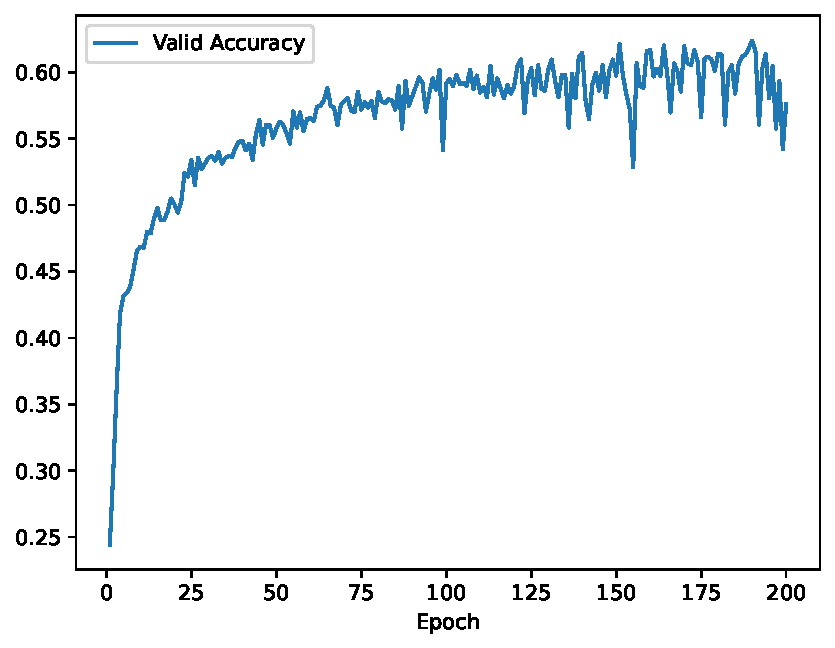
\includegraphics[width=\imagewidth]{q2/q2_2b_dropout_0.01-validation-accuracy.pdf} \\
                Test accuracy: 0.5763 \\
                Validation accuracy: 0.5762
            \item Dropout 0.25: \\
                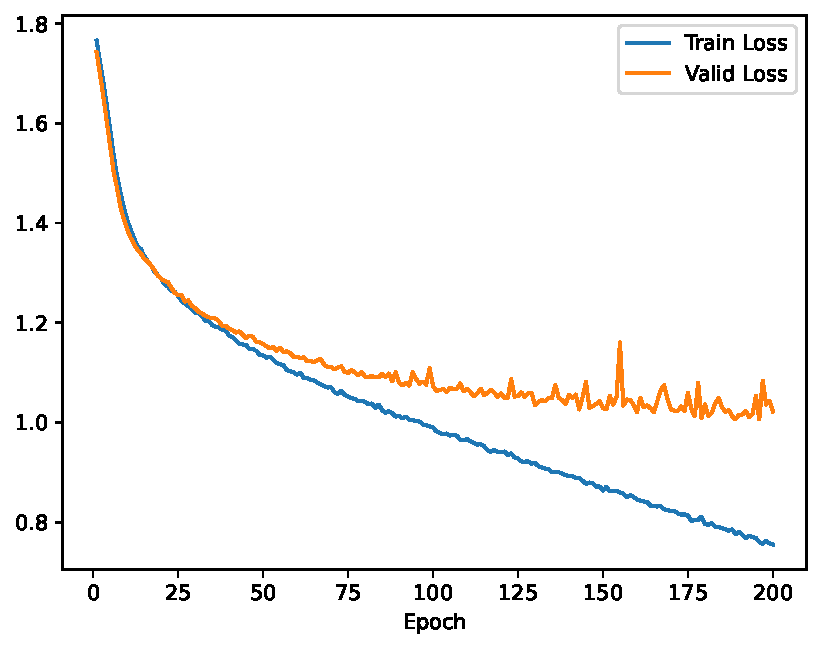
\includegraphics[width=\imagewidth]{q2/q2_2b_dropout_0.25-training-loss.pdf}
                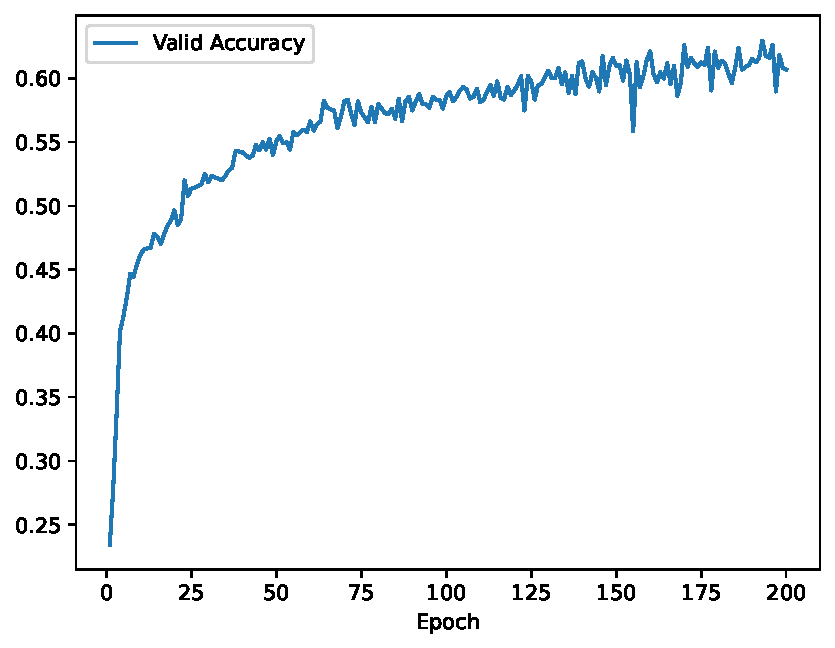
\includegraphics[width=\imagewidth]{q2/q2_2b_dropout_0.25-validation-accuracy.pdf} \\
                Test accuracy: 0.6063 \\
                Validation accuracy: 0.6068
            \newpage
            \item Dropout 0.5: \\
                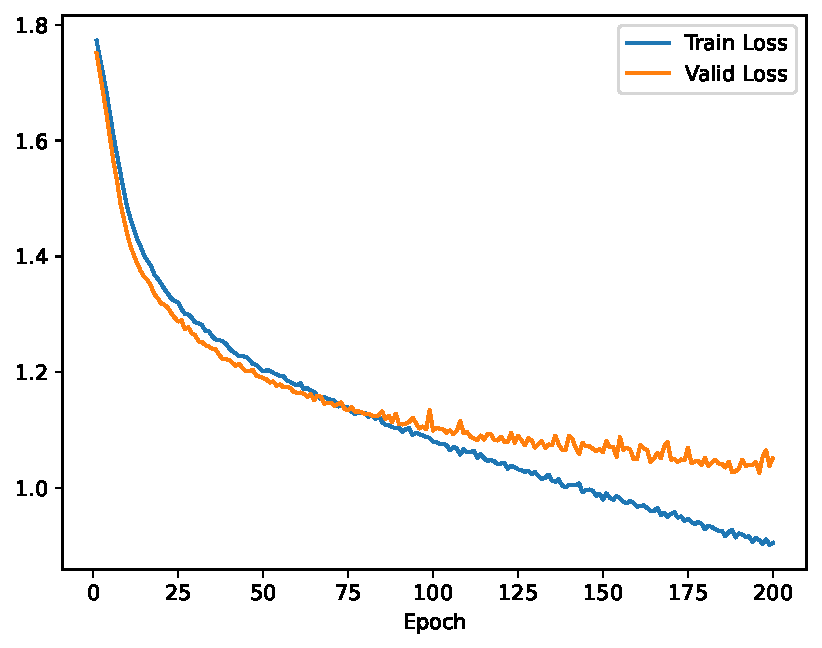
\includegraphics[width=\imagewidth]{q2/q2_2b_dropout_0.5-training-loss.pdf}
                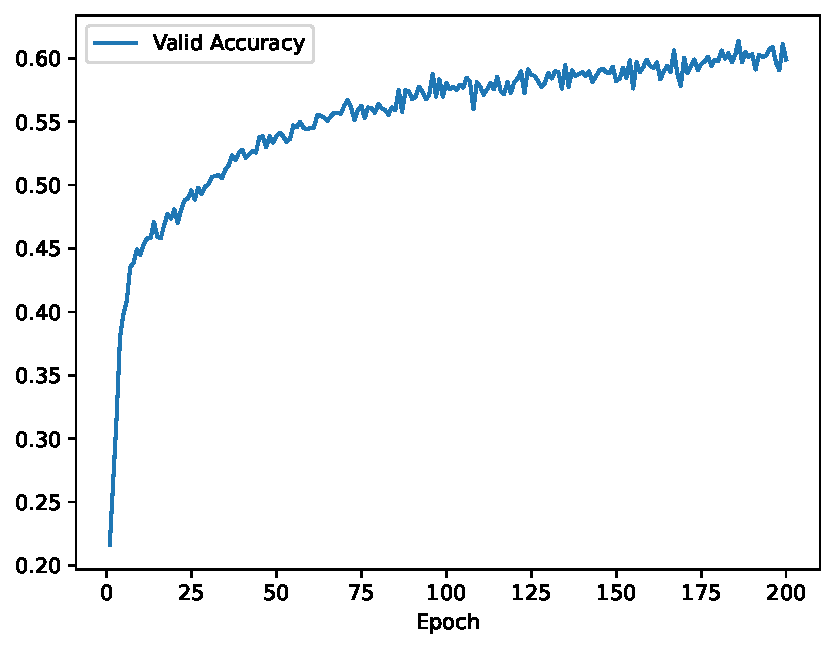
\includegraphics[width=\imagewidth]{q2/q2_2b_dropout_0.5-validation-accuracy.pdf} \\
                Test accuracy: 0.5950 \\
                Validation accuracy: 0.5990
        \end{itemize}
        The results demonstrate how dropout impacts both accuracy and learning behavior. A low dropout rate of 0.01 provided minimal regularization, which reduced its effectiveness in preventing overfitting. The validation loss curve is unstable, showing frequent spikes, and the model does not generalize well, likely overfitting the training data. \\
        When the dropout rate was increased to 0.25, the test and validation accuracies improved, meaning that this configuration struck a balance between regularization and performance. The loss curves for both training and validation exhibit smoother behavior compared to the previous setting, with smaller fluctuations, indicating effective prevention of overfitting and improved generalization. \\
        At a dropout rate of 0.5, the test and validation accuracy dropped slightly. The higher dropout rate introduced more regularization, which, while reducing overfitting, also caused the model to underfit slightly, resulting in a small reduction in accuracy. The loss curves show a slower decrease, especially in training loss, which reflects the challenge of learning with significant neuron dropout. \\
        In conclusion, a dropout rate of 0.25 provided the best performance, as it effectively balanced regularization and learning. A very low dropout rate of 0.01 led to overfitting, while a high dropout rate of 0.5 caused slight underfitting due to excessive regularization. This demonstrates that moderate dropout values are optimal for achieving both stability and accuracy.

    \newpage
    \subsection{2. c)}
        Plots of the train and validation losses (left) and the validation accuracy (right) as a function of the epoch number for the model trained with:
        \begin{itemize}
            \item Momentum 0.0: \\
                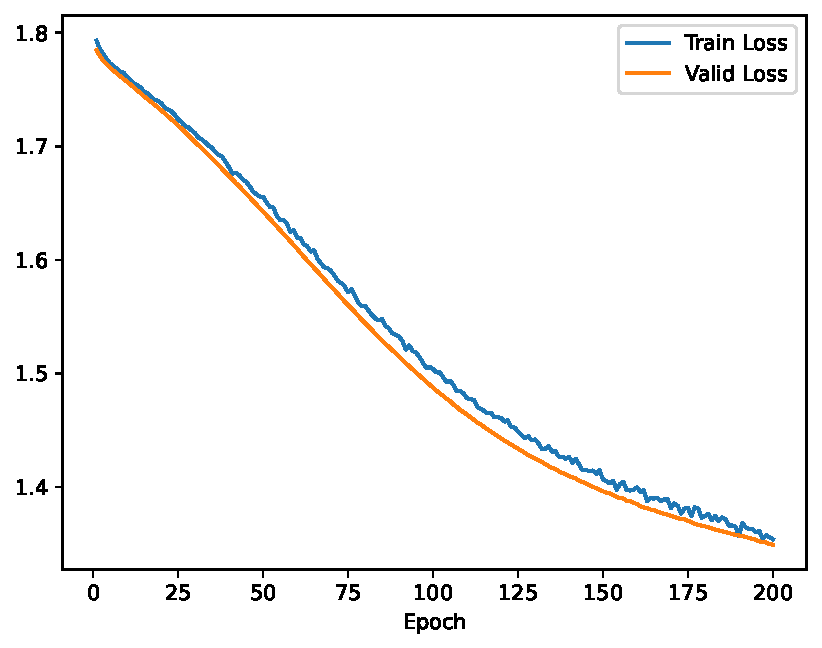
\includegraphics[width=\imagewidth]{q2/q2_2c_momentum_0.0-training-loss.pdf}
                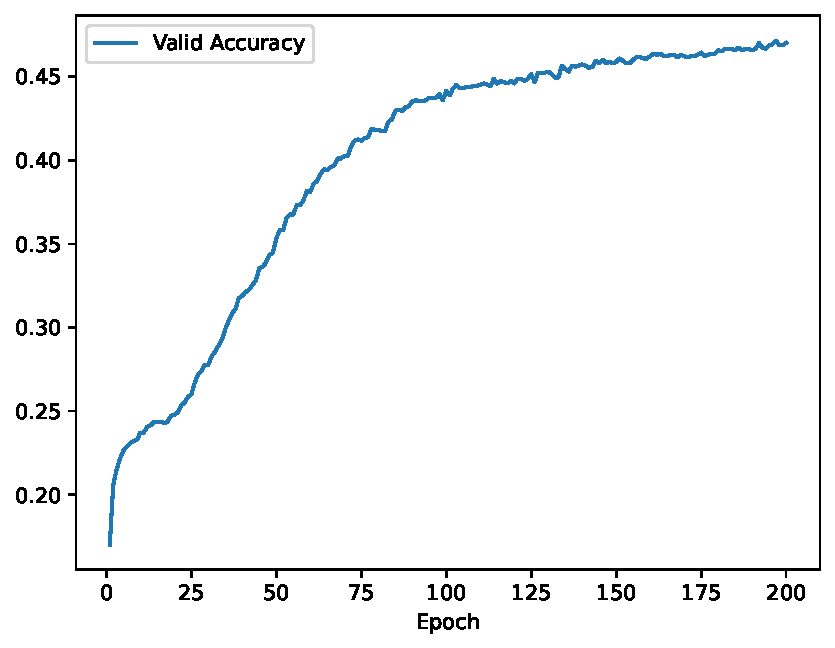
\includegraphics[width=\imagewidth]{q2/q2_2c_momentum_0.0-validation-accuracy.pdf} \\
                Test accuracy: 0.4887 \\
                Validation accuracy: 0.4701
            \item Momentum 0.9: \\
                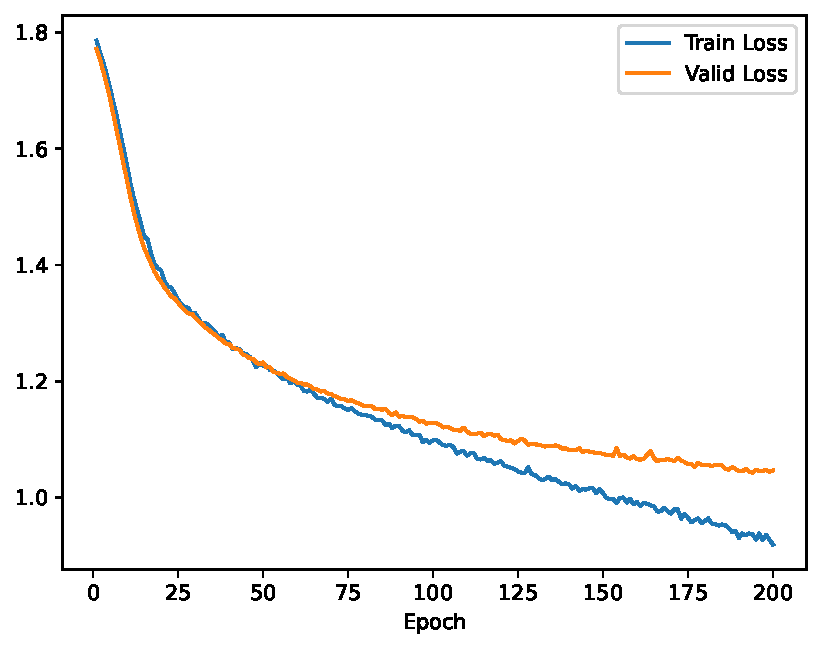
\includegraphics[width=\imagewidth]{q2/q2_2c_momentum_0.9-training-loss.pdf}
                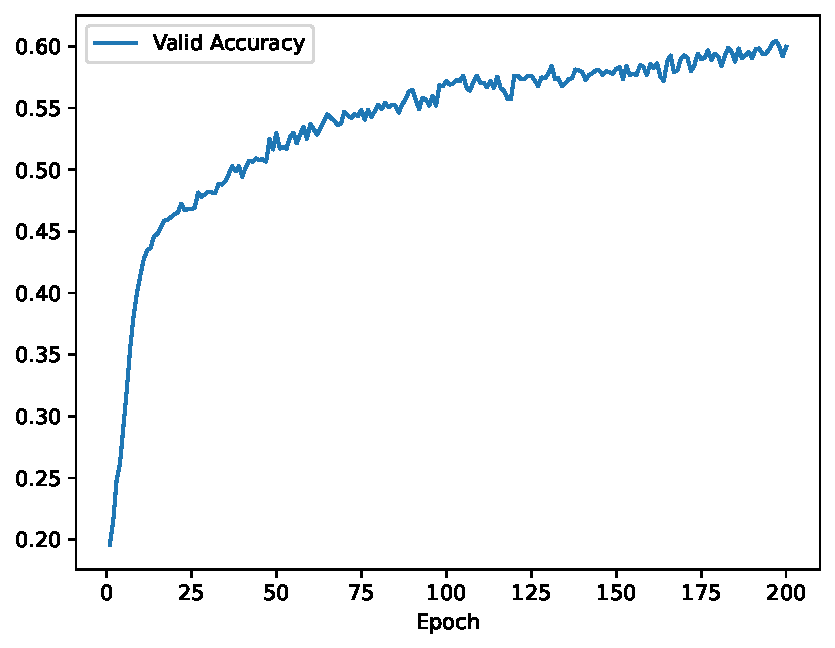
\includegraphics[width=\imagewidth]{q2/q2_2c_momentum_0.9-validation-accuracy.pdf} \\
                Test accuracy: 0.6010 \\
                Validation accuracy: 0.5997
        \end{itemize}
        Without momentum, the optimization process relied solely on the gradient updates from each step, leading to slower convergence. This can be observed in the loss curves, which decrease steadily but at a slower rate, showing that the model struggles to generalize effectively, resulting in lower accuracy. \\
        In contrast, with momentum set to 0.9, the test and validation accuracies improved significantly, as the momentum term accelerated the optimization process by smoothing the gradients, which increases the update in directions with stable gradient and helps overcome small variations and local minima. This led to faster convergence, as reflected in the sharper decrease in training loss and improved generalization, visible in the validation loss curve and higher accuracy scores. \\
        In conclusion, incorporating momentum improves convergence speed and generalization by smoothing the optimization trajectory, which leads to significantly better performance compared to training without momentum.


    \newpage
    \section{Question 3}
    \subsection{1.}
        We have a single hidden layer such that \(h = g(Wx+b)\), so, for each hidden unit \(j \in \{1,\ldots,K\}\):
        \[z_j = w_j^\top x + b_j,\]
        where \(w_j \in \mathbb{R}^D\) is the \(j\)-th row of \(W\), and \(b_j \in \mathbb{R}\). \\
        Then, once \(g(z) = z(1 - z) = z - z^2\), the hidden layer output is, for each unit:
        \[h_j = g(z_j) = z_j(1 - z_j) = z_j - z_j^2 \in \mathbb{R}^K.\]
        We want to determine how \(h_j\) depends on \(x\). \\
        First, we substitute \(z_j = w_j^\top x + b_j = b_j + \sum_{d=1}^D w_{j,d} x_d\) in the expression \(h_j = z_j - z_j^2\):
        \[h_j = z_j - z_j^2 = \left(b_j + \sum_{d=1}^D w_{j,d} x_d\right) - \left(b_j + \sum_{d=1}^D w_{j,d}x_d\right)^2 =\]
        \[= \left(b_j + \sum_{d=1}^D w_{j,d} x_d\right) - \left(b_j^2 + 2 b_j \sum_{d=1}^D w_{j,d}x_d + \sum_{d=1}^D\sum_{e=1}^D w_{j,d} w_{j,e} x_d x_e \right).\]
        Now, we can group the terms in this expression into constant, linear and quadratic parts:
       \begin{itemize}
            \item Constant term: \[b_j - b_j^2.\]
           
            \item Linear terms in \(x_d\): \\
                The linear terms come from \(\sum_d w_{j,d} x_d\) and \(- 2 b_j \sum_d w_{j,d} x_d\).\\
                Combining these:
                \[\text{Coefficient of } x_d: w_{j,d} - 2 b_j w_{j,d} = w_{j,d}(1 - 2b_j).\]
            
            \item Quadratic terms in \(x_d\) and \(x_e\): \\
                The quadratic terms come from \(-\sum_{d=1}^D\sum_{e=1}^D w_{j,d} w_{j,e} x_d x_e\).
                
                \begin{itemize}
                    \item When \(d = e\):
                        \[\text{Coefficient of } x_d^2: -w_{j,d}^2.\]
                    
                    \item When \(d \neq e\), we have \(x_d x_e\) terms. Note that for each pair \((d, e)\) with \(d < e\), there is a pair \((e, d)\), so we can group symmetric terms:
                        \[\sum_{d=1}^D \sum_{\substack{e = 1 \\ d \neq e}}^D w_{j,d} w_{j,e} x_d x_e = 2\sum_{1 \leq d < e \leq D} w_{j,d} w_{j,e} x_d x_e;\]
                        \[\text{Coefficient of } x_d x_e \text{ (with } d<e \text{): } -2 w_{j,d} w_{j,e}.\]
                \end{itemize}            
        \end{itemize}
        Hence:
        \[
        h_j = (b_j - b_j^2) \cdot 1 
        + \sum_{d=1}^D (w_{j,d}(1 - 2b_j)) x_d
        - \sum_{d=1}^D w_{j,d}^2 x_d^2
        - 2 \sum_{1 \leq d < e \leq D} w_{j,d} w_{j,e} x_d x_e.
        \]
        This is a linear function in terms of the following set of features:
        \[\phi(x) = \bigl(1,\; x_1,\ldots,x_D,\; x_1^2,\ldots,x_D^2,\; x_1x_2, x_1x_3,\ldots,x_{D-1}x_D \bigr)^\top.\]
        \(\phi(x)\) has \(1\) constant term, \(D\) linear terms and \(D + \frac{D(D-1)}{2}\) quadratic terms, so:
        \[\dim\phi(x) = 1 + D + D + \frac{D(D-1)}{2} = \frac{(D+1)(D+2)}{2}.\]
        Thus \(\phi: \mathbb{R}^D \to \mathbb{R}^{\frac{(D+1)(D+2)}{2}}\) and \(\phi\) is independent of \(\Theta\). \\
        Let \(\text{index}(x_d x_e)\) represent the indexes of the cross terms \(x_1x_2,x_1x_3,\ldots,x_{D-1}x_D\) in \(\phi(x)\). \\
        We now write \(h = (h_1,\ldots,h_K)^\top\) as:
        \[h = A_{\Theta} \phi(x).\]
        The matrix \(A_{\Theta}\) has size \(K \times \frac{(D+1)(D+2)}{2}\). The entries of each row \(j\) are:
        \begin{itemize}
            \item \([A_{\Theta}]_{j,1} = b_j - b_j^2\)
            \item \([A_{\Theta}]_{j,1+d} = w_{j,d}(1 - 2b_j), \quad \forall d \in \{1,\ldots,D\}\)
            \item \([A_{\Theta}]_{j,1+D+d} = -w_{j,d}^2, \quad \forall d \in \{1,\ldots,D\}\)
            \item \([A_{\Theta}]_{j,\text{index}(x_d x_e)} = -2 w_{j,d} w_{j,e}, \quad \forall \text{ index}(x_d x_e) \in \left\{1+2D+1,\ldots,\frac{(D+1)(D+2)}{2}\right\}\)
        \end{itemize}
        Here's a simplified representation of the matrix:
        \[
        A_{\Theta} =
        \begin{bmatrix}
        b_1 - b_1^2 & \cdots & w_{1,d}(1 - 2b_1) & \cdots & -w_{1,d}^2 & \cdots & -2 w_{1,d} w_{1,e} & \cdots \\
        \vdots      & \cdots & \vdots            & \cdots & \vdots     & \cdots & \vdots             & \cdots \\
        b_j - b_j^2 & \cdots & w_{j,d}(1 - 2b_j) & \cdots & -w_{j,d}^2 & \cdots & -2 w_{j,d} w_{j,e} & \cdots \\
        \vdots      & \cdots & \vdots            & \cdots & \vdots     & \cdots & \vdots             & \cdots \\
        b_K - b_K^2 & \cdots & w_{K,d}(1 - 2b_K) & \cdots & -w_{K,d}^2 & \cdots & -2 w_{K,d} w_{K,e} & \cdots
        \end{bmatrix}
        \]

    \subsection{2.}
        The model’s prediction is given by \(\hat{y} = v^\top h + v_0\). We substitute that in \(h = A_{\Theta} \phi(x)\):
        \[\hat{y} = v^\top (A_{\Theta} \phi(x)) + v_0 = (v^\top A_{\Theta}) \phi(x) + v_0 = (A_{\Theta}^\top v)^\top \phi(x) + v_0,\]
        where \(A_{\Theta}^\top v \in \mathbb{R}^\frac{(D+1)(D+2)}{2}\). Since \(\phi(x)\) has a constant first component \(\phi_1(x)=1\), the scalar \(v_0\) can be absorbed into the first component of this linear form. Specifically, define:
        \[c_{\Theta} := A_{\Theta}^\top v + v_0 e_1,\]
        where \(e_1 = (1,0,\ldots,0)^\top \in \mathbb{R}^{\frac{(D+1)(D+2)}{2}}\).
        With this definition, we have:
        \[\hat{y}(x; c_{\Theta}) = (A_{\Theta}^\top v + v_0 e_1)^\top \phi(x) = c_{\Theta}^\top \phi(x).\]
        Thus, \(\hat{y}\) is indeed a linear transformation of \(\phi(x)\), with parameter vector \(c_{\Theta}\). \\
        However, this does not mean it is a linear model in terms of the original parameters \(\Theta\). The parameter vector \(c_{\Theta}\) is a nonlinear function of \(\Theta = (W,b,v,v_0)\), so, although the mapping \(x \mapsto \hat{y}\) is linear in the feature space \(\phi(x)\), it is not linear in \(\Theta\). In other words, the model is equivalent to a linear model in a very high-dimensional feature space \(\phi(x)\), however, the mapping from \(\Theta\) to \(c_{\Theta}\) involves products and squares of the elements of \(W\) and \(b\), which makes the dependency on \(\Theta\) highly nonlinear.

    \newpage
    \subsection{3.}
        We are given \(c \in \mathbb{R}^{\frac{(D+1)(D+2)}{2}}\) and want to find parameters \(\Theta\) such that \(\|c_{\Theta}-c\|<\epsilon\).\\
        Let's break down \(c\):
        \[c = c_1 e_1 + \tilde{c},\]
        where \(e_1 = (1,0,\ldots,0)^\top \in \mathbb{R}^{\frac{(D+1)(D+2)}{2}}\) and \(\tilde{c} = (0, c_2, \ldots, c_{\frac{(D+1)(D+2)}{2}})\). \\
        We set \(v_0 = c_1\), so that the constant part of \(c_{\Theta}\) is aligned with \(c_1\). Now we need to match the remaining \(\tilde{c}\) with \(A_{\Theta}^\top\):
        \[c_{\Theta} = A_{\Theta}^\top v + v_0 e_1 = A_{\Theta}^\top v + c_1 e_1
        \quad \Leftrightarrow \quad A_{\Theta}^\top v = c_{\Theta} - c_1 e_1.\]
        Hence we want to solve:
        \[A_{\Theta}^\top v = c - c_1 e_1 = \tilde{c}.\]
        Let's consider the construction of \(A_\Theta\) from \((W,b)\). Since \(A_\Theta\) depends continuously on \((W,b)\), we can start with an arbitrary \((W,b)\), compute the corresponding \(A_\Theta\), and then, if \(A_\Theta\) is not invertible or well-conditioned, use the fact that any matrix is \(\epsilon\)-close to a non-singular matrix. In other words, we can adjust \((W,b)\) slightly so that the resulting \(A_\Theta\) is invertible or at least well-conditioned. \\
        Since \(A_\Theta\) is chosen to be non-singular (or very close to it), we can perform a QR decomposition:
        \[A_\Theta = Q R,\]
        where \(Q\) is \(K\times \frac{(D+1)(D+2)}{2}\) with orthonormal columns and \(R\) is \(\frac{(D+1)(D+2)}{2} \times \frac{(D+1)(D+2)}{2}\) invertible.
        If \(A_\Theta\) is not square but tall, we can consider a suitable sub-block or use the Moore-Penrose pseudoinverse. The main idea remains: we can ensure \(A_\Theta\) has full column rank and hence \(R\) is invertible. \\
        Thus:
        \[A_\Theta^\top v = \tilde{c} \quad \Leftrightarrow \quad (Q R)^\top v = \tilde{c} \quad \Leftrightarrow \quad R^\top Q^\top v = \tilde{c}.\]
        Since \(R\) is invertible, we can solve:
        \[R^\top Q^\top v = \tilde{c} \quad \Leftrightarrow \quad Q^\top v = (R^\top)^{-1} \tilde{c}.\]
        Then:
        \[Q^\top v = (R^\top)^{-1} \tilde{c} \quad \Rightarrow \quad v = Q (R^\top)^{-1} \tilde{c}.\]
        This gives an explicit way to solve for \(v\). \\
        This way, we can compute parameters \(\Theta = (W,b,v,v_0)\) for which \(c_\Theta\) is arbitrarily close to \(c\). Hence, up to \(\epsilon\)-precision, we can parameterize the model directly by \(c\) instead of \(\Theta\).

    \newpage
    \subsection{4.}
        The squared loss over a training set \(\mathcal{D} = \{(x_n,y_n)\}_{n=1}^N\) is:
        \[L(c_\Theta; \mathcal{D}) = \frac{1}{2}\sum_{n=1}^N (\hat{y}(x_n; c_\Theta) - y_n)^2.\]
        We substitute \(\hat{y}(x_n; c_\Theta) = c_\Theta^\top \phi(x_n)\) on that expression, getting:
        \[L(c_\Theta; \mathcal{D}) = \frac{1}{2}\sum_{n=1}^N (c_\Theta^\top \phi(x_n) - y_n)^2.\]
        Let \(\Phi \in \mathbb{R}^{N \times \frac{(D+1)(D+2)}{2}}\) be the design matrix, where each row is \(\phi(x_n)^\top\):
        \[\Phi = \begin{bmatrix} \phi(x_1)^\top \\ \vdots \\ \phi(x_N)^\top \end{bmatrix}
        \quad ; \quad
        \Phi c_\Theta = \begin{bmatrix} \phi(x_1)^\top c_\Theta \\ \vdots \\ \phi(x_N)^\top c_\Theta \end{bmatrix}
        = \begin{bmatrix} c_\Theta^\top \phi(x_1) \\ \vdots \\ c_\Theta^\top \phi(x_N) \end{bmatrix}
        \quad ; \quad
        y = \begin{bmatrix} y_1 \\ \vdots \\ y_N \end{bmatrix}.\]
        Then the loss is:
        \[L(c_\Theta; \mathcal{D}) = \frac{1}{2}\| \Phi c_\Theta - y \|_2^2.\]
        Since this is now a standard linear least squares problem, there is a closed-form solution, provided \(\Phi^\top \Phi\) is invertible. With \(N > \frac{(D+1)(D+2)}{2}\) and the assumption that \(\{\phi(x_n)\}_{n=1}^N\) are sufficiently rich (for example, if the original \(\{x_n\}_{n=1}^N\) are linearly independent and well-chosen), \(\Phi^\top \Phi\) will typically be invertible, and the solution will be:
        \[\hat{c}_\Theta = (\Phi^\top \Phi)^{-1} \Phi^\top y.\]
        For a general feedforward neural network with nonlinear activations like sigmoid, ReLU, or tanh, global minimization is usually intractable, because the loss surface is non-convex and there is no known closed-form solution. Finding the global minimum typically involves non-linear optimization techniques such as gradient descent, and the problem can have many local minima, saddle points, and other complicated phenomena. \\
        The key in our problem is the chosen activation \(g(z) = z(1-z)\). This activation is a quadratic function in terms of \(x\), once you substitute \(z = Wx + b\). Because of this, the hidden layer outputs can be expressed as linear functions of a fixed polynomial feature mapping \(\phi(x)\). Hence, the entire model becomes linear in these augmented features, turning a typically non-linear, non-convex problem into a linear, convex one with a closed-form solution.

\end{document}